%%%%%%%%%%%%%%%%%%%%%%%%%%%%%%%%%%%%%%%%%
% Beamer Presentation
% LaTeX Template
% Version 1.0 (10/11/12)
%
% This template has been downloaded from:
% http://www.LaTeXTemplates.com
%
% License:
% CC BY-NC-SA 3.0 (http://creativecommons.org/licenses/by-nc-sa/3.0/)
%
%%%%%%%%%%%%%%%%%%%%%%%%%%%%%%%%%%%%%%%%%

%----------------------------------------------------------------------------------------
%	PACKAGES AND THEMES
%----------------------------------------------------------------------------------------

\documentclass{beamer}

\usepackage{tikz}
\usetikzlibrary{arrows,automata,positioning}

\mode<presentation> {

% The Beamer class comes with a number of default slide themes
% which change the colors and layouts of slides. Below this is a list
% of all the themes, uncomment each in turn to see what they look like.

%\usetheme{default}
%\usetheme{AnnArbor}
%\usetheme{Antibes}
%\usetheme{Bergen}
%\usetheme{Berkeley}
%\usetheme{Berlin}
%\usetheme{Boadilla}
%\usetheme{CambridgeUS}
%\usetheme{Copenhagen}
%\usetheme{Darmstadt}
%\usetheme{Dresden}
%\usetheme{Frankfurt}
%\usetheme{Goettingen}
%\usetheme{Hannover}
%\usetheme{Ilmenau}
%\usetheme{JuanLesPins}
%\usetheme{Luebeck}
%\usetheme{Madrid}
%\usetheme{Malmoe}
%\usetheme{Marburg}
\usetheme{Montpellier}
%\usetheme{PaloAlto}
%\usetheme{Pittsburgh}
%\usetheme{Rochester}
%\usetheme{Singapore}
%\usetheme{Szeged}
%\usetheme{Warsaw}

% As well as themes, the Beamer class has a number of color themes
% for any slide theme. Uncomment each of these in turn to see how it
% changes the colors of your current slide theme.

%\usecolortheme{albatross}
%\usecolortheme{beaver}
%\usecolortheme{beetle}
%\usecolortheme{crane}
\usecolortheme{dolphin}
%\usecolortheme{dove}
%\usecolortheme{fly}
%\usecolortheme{lily}
%\usecolortheme{orchid}
%\usecolortheme{rose}
%\usecolortheme{seagull}
%\usecolortheme{seahorse}
%\usecolortheme{whale}
%\usecolortheme{wolverine}

%\setbeamertemplate{footline} % To remove the footer line in all slides uncomment this line
%\setbeamertemplate{footline}[page number] % To replace the footer line in all slides with a simple slide count uncomment this line

\setbeamertemplate{navigation symbols}{} % To remove the navigation symbols from the bottom of all slides uncomment this line
}

\usepackage{graphicx} % Allows including images
\usepackage{booktabs} % Allows the use of \toprule, \midrule and \bottomrule in tables

%----------------------------------------------------------------------------------------
%	TITLE PAGE
%----------------------------------------------------------------------------------------

\title[INF210]{INF210 Overview} % The short title appears at the bottom of every slide, the full title is only on the title page

\author{Åsmund Kløvstad} % Your name
\institute[UiB] % Your institution as it will appear on the bottom of every slide, may be shorthand to save space
{
Universitetet i Bergen \\ % Your institution for the title page
}
\date{\today} % Date, can be changed to a custom date

\begin{document}

\begin{frame}
\titlepage % Print the title page as the first slide
\end{frame}

% \begin{frame}
% \frametitle{Overview} % Table of contents slide, comment this block out to remove it
% \tableofcontents % Throughout your presentation, if you choose to use \section{} and \subsection{} commands, these will automatically be printed on this slide as an overview of your presentation
% \end{frame}

%----------------------------------------------------------------------------------------
%	PRESENTATION SLIDES
%----------------------------------------------------------------------------------------

%------------------------------------------------
\section{STS, LTS and Finite Automata} % Sections can be created in order to organize your presentation into discrete blocks, all sections and subsections are automatically printed in the table of contents as an overview of the talk
%------------------------------------------------

\begin{frame}
\frametitle{State Transition Systems}
\begin{itemize}
\item a tuple $(S, R)$
  \item $S = \{s_0,s_1...\}$
\item $R \subseteq S \times S$
  \item example: switch = $(\{s_0, s_1\}, \{ s_0 \times s_1, s_1 \times s_0\})$
\end{itemize}

\begin{figure}
  \centering
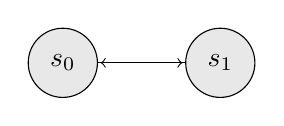
\begin{tikzpicture}[shorten >=1pt,node distance=2cm,on grid,auto] 
  \tikzstyle{every state}=[fill={rgb:black, 1;white,10}]

  \node[state] (s_0)                {$s_0$};
  \node[state] (s_1) [right of=s_0] {$s_1$};

  \path[->]
  (s_0) edge node {} (s_1)
  (s_1) edge node {} (s_0);
\end{tikzpicture}
  \end{figure}
\end{frame}

%------------------------------------------------

\begin{frame}
\frametitle{Important Properties of STSs}
\begin{itemize}
\item if a state has no rules going \textit{from} it, it is a \textbf{terminal
    state}.
\item if there is a sequence of steps from state $a$ to state $b$, $b$ is
  \textbf{reachable} from $a$. Write $R^*(a, b)$.
\item if $R$ is a function (in the set theory sense), the STS is \textbf{deterministic}.
\item if all paths eventually converge (clarify/formalize?) the STS is \textbf{confluent}.
\item switch is deterministic and confluent, and has no terminal states.
\end{itemize}
\end{frame}

%------------------------------------------------

\begin{frame}
\frametitle{Labeled Transition Systems}
\begin{block}{Syntax}
\begin{itemize}
\item extends STSs with labels
\item a 3-tuple $(S, L, R)$.
\item $R \subseteq S \times L \times S$, often written $s \xrightarrow{a} s'$
\end{itemize}
\end{block}
\begin{block}{Reachability}
\begin{itemize}
\item consider the STS $(S_L, R_L)$ with:
  \begin{itemize}
  \item $S_L = S \times L^*$
  \item $s \times l \cdot \mathbf{w} \rightarrow s' \times \mathbf{w} \in R_L$
    iff $s \xrightarrow{l} s' \in R$ 
   \end{itemize}
\item $s'$ is reachable from $s$ by $\mathbf{w}$ if $s' \times \lambda$ is
      reachable from $s \times \mathbf{w}$.
    \item write $s \times \mathbf{w} \vdash_{R}^* s' \times \lambda$
\end{itemize}
\end{block}
\end{frame}

%------------------------------------------------

\begin{frame}
\frametitle{Finite Automata}
\begin{itemize}
\item $M = (\Sigma, Q, q_0, \Upsilon, F)$
\item a finite LTS with initial and final states
\item the language accepted by $M$ is $L_M = \{\mathbf{w} \; | \; q_0 \times
  \mathbf{w} \vdash_{\Upsilon}^* q_i \times \lambda \text{ and } q_i \in F\}$
\end{itemize}
\end{frame}


%------------------------------------------------
\section{Regular Languages}
%------------------------------------------------

%------------------------------------------------

\begin{frame}
\frametitle{Kleene's Theorem}
\begin{theorem}
  a language is regular $\iff$ it is accepted by a finite automata
\end{theorem}
\begin{block}{$\Rightarrow$}
Construct FAs to accept the empty language, $\{\lambda\}$ and singleton
languages. Then construct FAs for union, concatenation, and Kleene star.
\end{block}

\begin{block}{$\Leftarrow$}
Define $R(i, k, j) = \{\mathbf{w} \; | \; q_j \text{ is reachable from } q_i
\text{ without visiting } q_m \text{ with } m \geq k\}$\\

Then show $R(i, k+1, j) = R(i, k, j) \cup R(i, k, k) \cdot R(k, k, k)^* \cdot
R(k, k, j)$
\end{block}
\end{frame}

\end{document} 